% S^1 covered by two open arcs U (blue) and V (red) for Mayer-Vietoris.
% Source: book/tex/homology/long-exact.tex (§ Application: Mayer-Vietoris).
\documentclass[border=2mm]{standalone}
\usepackage{tikz}
\begin{document}
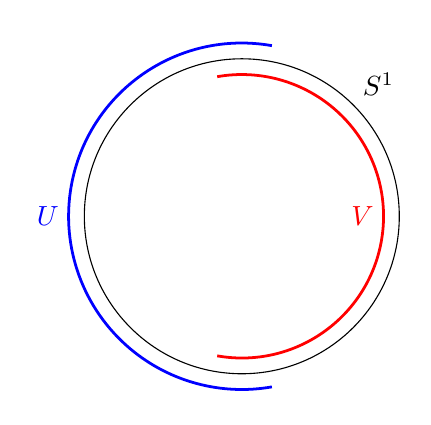
\begin{tikzpicture}[scale=2]
  \draw (0,0) circle (1);
  \node at (45:1) [above right] {$S^1$};
  \draw[red, line width=1pt] (-100:0.9) arc (-100:100:0.9);
  \node[red, left] at (0:0.9) {$V$};
  \draw[blue, line width=1pt] (80:1.1) arc (80:280:1.1);
  \node[blue, left] at (180:1.1) {$U$};
\end{tikzpicture}
\end{document}
